\chapter{INDEX.}

\begin{figure}[h!]
\centering
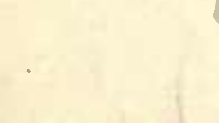
\includegraphics[width=0.8\textwidth]{../imagenes/pagina_018_fig_01.png}
\caption{Figura de la página 18}
\end{figure}

\begin{figure}[h!]
\centering

\includegraphics[width=0.8\textwidth]{../imagenes/pagina_018_fig_02.png}
\caption{Figura de la página 18}
\end{figure}

\begin{figure}[h!]
\centering

\includegraphics[width=0.8\textwidth]{../imagenes/pagina_018_fig_03.png}
\caption{Figura de la página 18}
\end{figure}

\begin{figure}[h!]
\centering
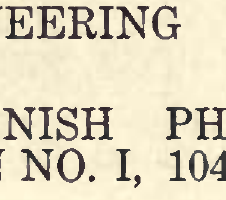
\includegraphics[width=0.8\textwidth]{../imagenes/pagina_018_fig_04.png}
\caption{Figura de la página 18}
\end{figure}

\begin{figure}[h!]
\centering
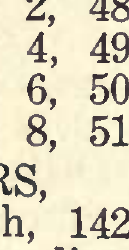
\includegraphics[width=0.8\textwidth]{../imagenes/pagina_018_fig_05.png}
\caption{Figura de la página 18}
\end{figure}

\begin{figure}[h!]
\centering
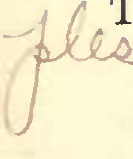
\includegraphics[width=0.8\textwidth]{../imagenes/pagina_018_fig_06.png}
\caption{Figura de la página 18}
\end{figure}

\begin{figure}[h!]
\centering
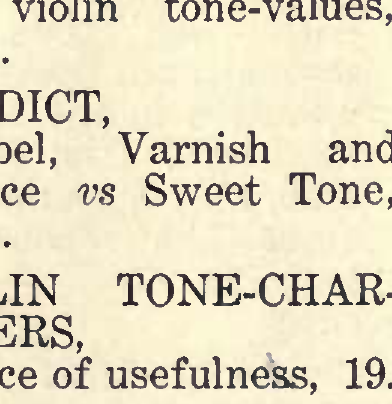
\includegraphics[width=0.8\textwidth]{../imagenes/pagina_018_fig_07.png}
\caption{Figura de la página 18}
\end{figure}

\begin{figure}[h!]
\centering
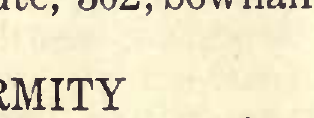
\includegraphics[width=0.8\textwidth]{../imagenes/pagina_018_fig_08.png}
\caption{Figura de la página 18}
\end{figure}

\begin{figure}[h!]
\centering
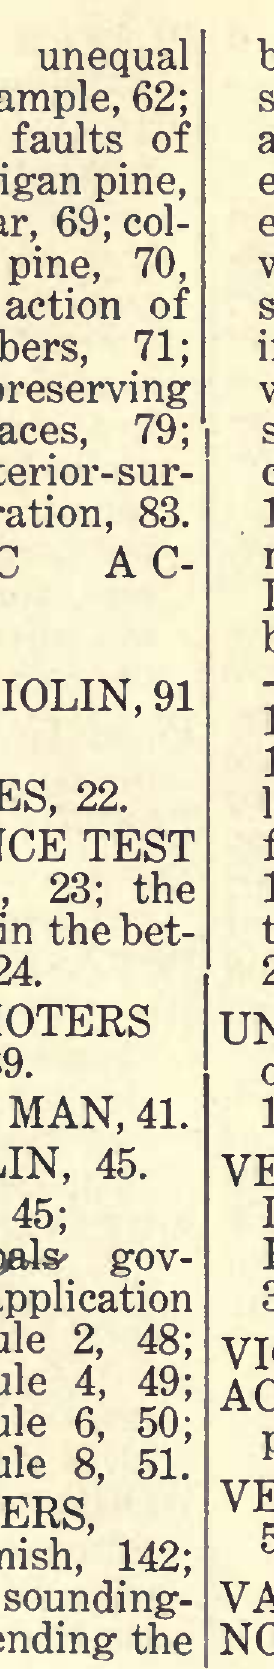
\includegraphics[width=0.8\textwidth]{../imagenes/pagina_018_fig_09.png}
\caption{Figura de la página 18}
\end{figure}

\begin{figure}[h!]
\centering
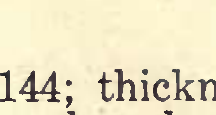
\includegraphics[width=0.8\textwidth]{../imagenes/pagina_018_fig_10.png}
\caption{Figura de la página 18}
\end{figure}

\begin{figure}[h!]
\centering

\includegraphics[width=0.8\textwidth]{../imagenes/pagina_018_fig_11.png}
\caption{Figura de la página 18}
\end{figure}

\begin{figure}[h!]
\centering
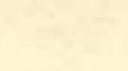
\includegraphics[width=0.8\textwidth]{../imagenes/pagina_018_fig_12.png}
\caption{Figura de la página 18}
\end{figure}

violins, 61; unequal back, 144; thickness of skrinkage, example, 62; sounding-board, 144; example, 63; faults of arching, 147; high a"rch, pine, 66; Michigan pine, example, 148; laws gov- 67; white cedar, 69; col- erning lines, of sound- or changes in pine, 70, wave travel, 151; un- independent action of solved problem in arch- contiguous fibers, 71; ing, 152, the bar, 152; pathetic, 78; preserving wolf caused by mal-po- interior surfaces, 79; sition of bar, 153; wolf example of interior-sur- I caused by graduation, face disintegration, 83. 154; position of bar di- SYMPATHETIC A C- minishing power of the TION, 108; D, 158; the post, 1QO; the law of, 109. bridge, 164; the finger- SWEET OLD VIOLIN, 91 -board, 165; the strings, THE KING, 181; re- enforce block, TWO 20. 175; the trembling vio- MISTAKES, 22. lin, 181; interior sur- TONE-DISTANCE TEST faces, 185; the exits, out of doors, 23; the 187; depth of ribs, 199; listening ear in the bet- the mute, 302;bowhair, ter position, 24. 202. TRADE PROMOTERS UNIFORMITY industry of, 39. of violin tone- values, TWO-DOLLAR MAN, 41. 131. THOU, VIOLIN, 45. VERDICT, TONE-PITCH, 45; Label, Varnish and -"'. eight principals' gov- Price vs Sweet Tone, erning, 46; application 305. rulel, 48; rule 2, 48; VIOLIN TONE-CHAR- rule 3, 49; rule 4, 49; ACTERS, ruleS, 50; rule 6, 50; place of usefulness, 19. rule 7, 51; rule 8, 51. VENEERING WORKS, TONE-MODIFIERS, list, 141; varnish, 142; 53. bending the sounding- VARNISH PHENOME- board, 143; bending the NON NO. I, 104.\\
\begin{figure}[h!]
\centering
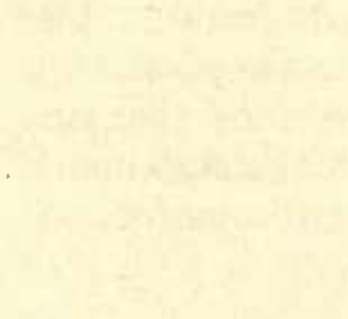
\includegraphics[width=0.8\textwidth]{../imagenes/pagina_019_fig_01.png}
\caption{Figura de la página 19}
\end{figure}

\begin{figure}[h!]
\centering
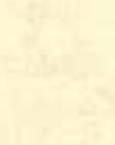
\includegraphics[width=0.8\textwidth]{../imagenes/pagina_019_fig_02.png}
\caption{Figura de la página 19}
\end{figure}

\begin{figure}[h!]
\centering
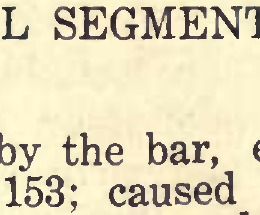
\includegraphics[width=0.8\textwidth]{../imagenes/pagina_019_fig_03.png}
\caption{Figura de la página 19}
\end{figure}

\begin{figure}[h!]
\centering
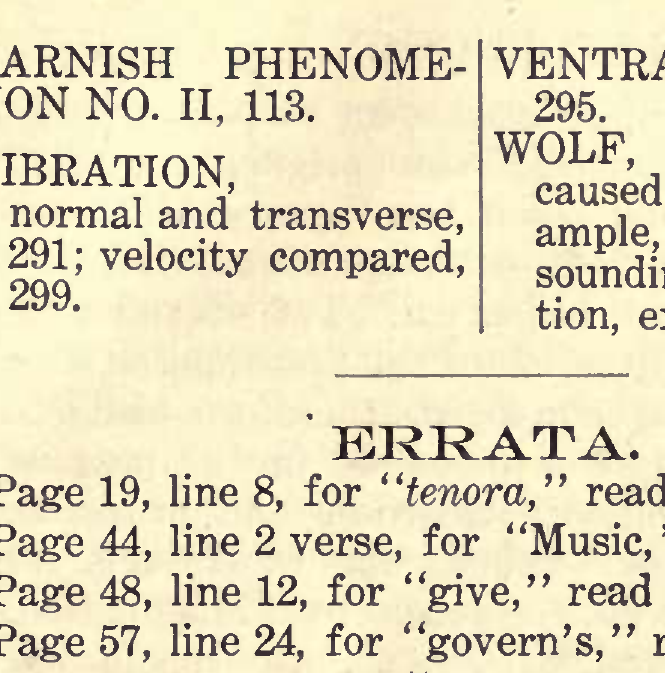
\includegraphics[width=0.8\textwidth]{../imagenes/pagina_019_fig_04.png}
\caption{Figura de la página 19}
\end{figure}

INDEX. VARNISH PHENOME- VENTRAL SEGMENTS, NON NO. II, 113. 295. WOLF, VIBRATION, caused by the bar, ex- normal and transverse, ample, 153; caused by 291; velocity compared, sounding-board gradua- 299. tion, example, 154. ERRATA. Page 19, line 8, for "tenora," read tenoro. Page 44, line 2 verse, for "Music," read Music's. Page 48, line 12, for "give," read gives. Page 57, line 24, for "govern's," read governs. Page 96, line 14, for "a basso,'' read a bassa. Page 173, line 1, for "diminish," read increase. Page 216, line 20, for "purfing," read purfling. Page 217, lines 1, 13, for "purfing," read purfling. Page 297, line 3, for "MOVEMENT," read MOVEMENTS.\\
XI\\
\begin{figure}[h!]
\centering

\includegraphics[width=0.8\textwidth]{../imagenes/pagina_020_fig_01.png}
\caption{Figura de la página 20}
\end{figure}

\begin{figure}[h!]
\centering
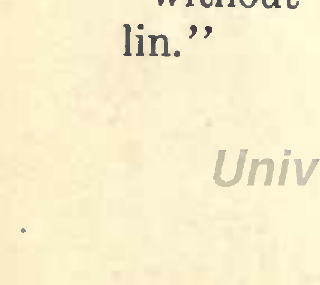
\includegraphics[width=0.8\textwidth]{../imagenes/pagina_020_fig_02.png}
\caption{Figura de la página 20}
\end{figure}

\begin{figure}[h!]
\centering
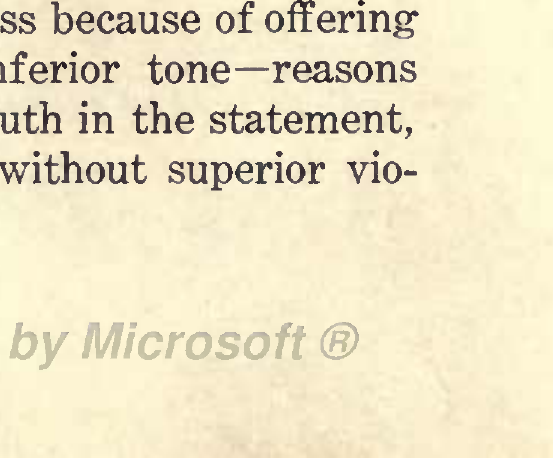
\includegraphics[width=0.8\textwidth]{../imagenes/pagina_020_fig_03.png}
\caption{Figura de la página 20}
\end{figure}

\begin{figure}[h!]
\centering
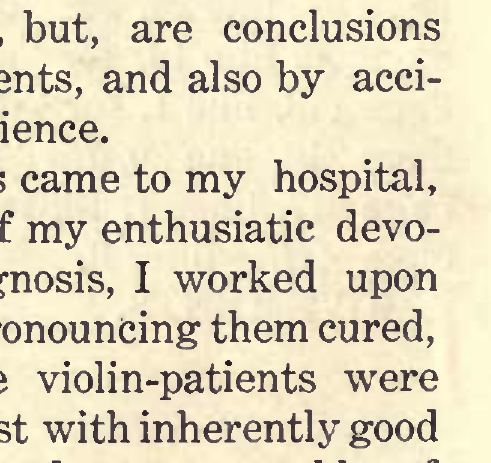
\includegraphics[width=0.8\textwidth]{../imagenes/pagina_020_fig_04.png}
\caption{Figura de la página 20}
\end{figure}

\begin{figure}[h!]
\centering
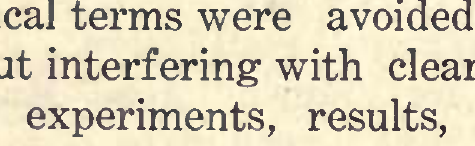
\includegraphics[width=0.8\textwidth]{../imagenes/pagina_020_fig_05.png}
\caption{Figura de la página 20}
\end{figure}

\begin{figure}[h!]
\centering
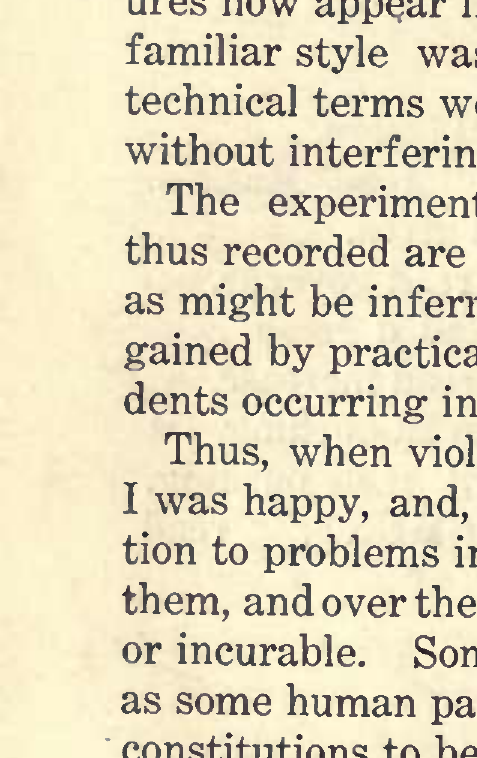
\includegraphics[width=0.8\textwidth]{../imagenes/pagina_020_fig_06.png}
\caption{Figura de la página 20}
\end{figure}

\begin{figure}[h!]
\centering
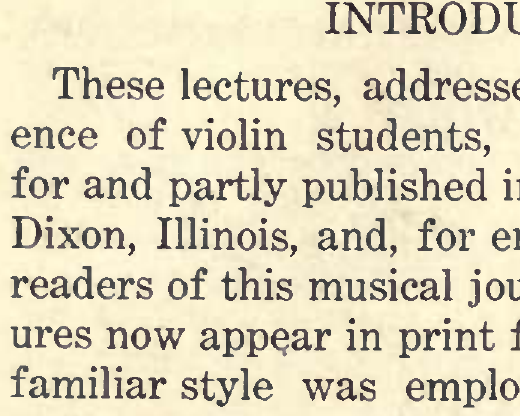
\includegraphics[width=0.8\textwidth]{../imagenes/pagina_020_fig_07.png}
\caption{Figura de la página 20}
\end{figure}

\begin{figure}[h!]
\centering
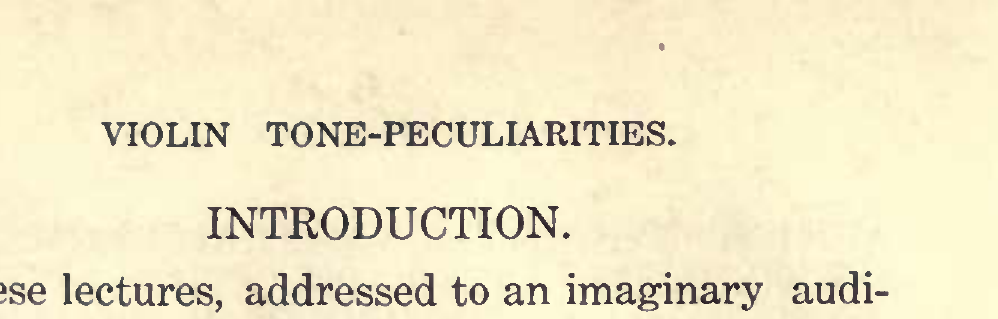
\includegraphics[width=0.8\textwidth]{../imagenes/pagina_020_fig_08.png}
\caption{Figura de la página 20}
\end{figure}

\begin{figure}[h!]
\centering
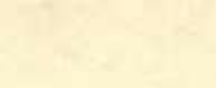
\includegraphics[width=0.8\textwidth]{../imagenes/pagina_020_fig_09.png}
\caption{Figura de la página 20}
\end{figure}

\section{VIOLIN TONE-PECULIARITIES.}

INTRODUCTION. These lectures, addressed to an imaginary audi- ence of violin students, were originally written for and partly published in the Western Musician, Dixon, Illinois, and, for entertainment of the many readers of this musical journal. Two of the lect- ures now appear in print for the first time. As a familiar style was employed, therefore abstruse technical terms were avoided as far as possible without interfering with clearness and precision. The experiments, results, and conclusions, as thus recorded are not romances of the imagination, as might be inferred at first, but, are conclusions gained by practical experiments, and also by acci- dents occurring in my experience. Thus, when violin patients came to my hospital, I was happy, and, because of my enthusiatic devo- tion to problems in tone-diagnosis, I worked upon them, and over them, until pronouncing them cured, or incurable. Some of those violin-patients were as some human patients, blest with inherently good constitutions to begin with, and, were capable of receiving enhanced tone values from careful adjust- ment of tone-modifying factors, while some of them were so inherently bad from the day they were named "violin," (misnamed,) that only noisy tone was their inheritance; yet, noisy tone made "inter- esting cases" of the latter class because of offering incontestable reasons for inferior tone reasons conclusively demonstrating truth in the statement, "without superior material, without superior vio- lin."

\section{xn}

\begin{figure}[h!]
\centering
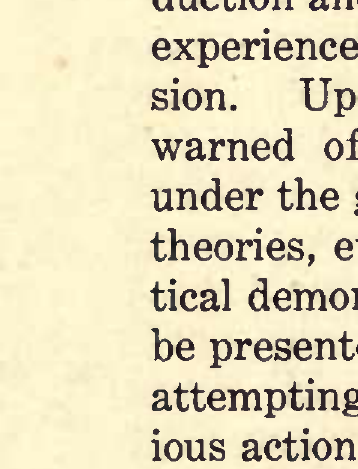
\includegraphics[width=0.8\textwidth]{../imagenes/pagina_021_fig_01.png}
\caption{Figura de la página 21}
\end{figure}

\begin{figure}[h!]
\centering
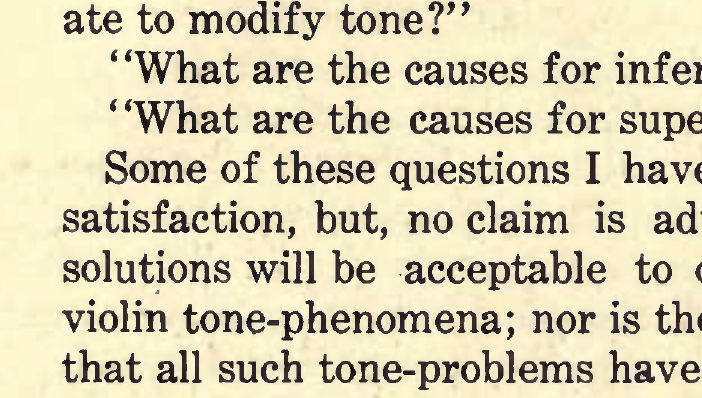
\includegraphics[width=0.8\textwidth]{../imagenes/pagina_021_fig_02.png}
\caption{Figura de la página 21}
\end{figure}

\begin{figure}[h!]
\centering
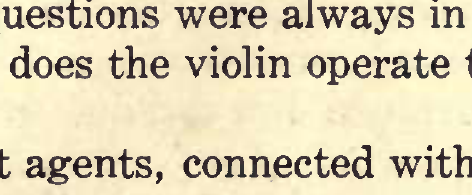
\includegraphics[width=0.8\textwidth]{../imagenes/pagina_021_fig_03.png}
\caption{Figura de la página 21}
\end{figure}

\section{VIOLIN TONE-PECULIARITIES.}

Throughout my period for active work, the fol- lowing questions were always in view: "How does the violin operate to produce musical sound?" 'What ' agents, connected with the violin, oper- ate to modify tone?" "What are the causes for inferior violin tone?" "What are the causes for superior violin tone?" Some of these questions I have solved to my own satisfaction, but, no claim is advanced that such solutions will be acceptable to other students of violin tone-phenomena; nor is the claim advanced that all such tone-problems have received solution. Some of my conclusions are at variance with con- clusions of noted scientific investigators, but, for my own conclusions, infallibility is not claimed. To err is human. To follow error is also human. Thus, I followed a scientific conclusion concerning pro- duction and modification of violin tone requiring experiences of twenty-five years to dispel the delu- sion. Upon this ground, the violin student is warned of danger in following abstract theory under the guise of science. It is my belief that theories, even when based upon oft-repeated prac- tical demonstrations upon various violins, should be presented only as conclusions of an individual attempting solution of a problem wherein capric- ious action of wood has ever been, is now, and for- ever may remain an unknown quantity; and, I pre- sent the thought that such unknown quantity is the reason why science meets defeat in attempting to build a violin to order.
